\chapter{Testing}
\label{chap:testing}
To ensure that the platform works correctly and doesn't break any connectivity outside the remit of the automation platform, several tests were devised. Virtual Machines attached directly to hardware \gls{nic}s were used. These \gls{vm}s were connected as follows:

\begin{table}[htbp]
    \centering
    \begin{tabular}{@{} c c @{}}
        \toprule
        \textbf{Test VM}     & \textbf{Fabric Port} \\
        \midrule
        \texttt{1} & \texttt{FEX101/1}    \\
        \texttt{2} & \texttt{FEX102/1}    \\
        \texttt{3} & \texttt{FEX103/1}    \\
        \bottomrule
    \end{tabular}
    \caption{Test VM fabric connections}
\end{table}

This will allow for the testing of communication between different fabric nodes to determine if the \gls{aci} fabric has been provisioned correctly. Access to the internet from the test VMs will also be tested to ensure that the virtual router has been provisioned correctly. Connectivity to the project's terminal servers will also be tested from the test VMs.
The automation platform was setup as follows:

\begin{table}[htbp]
    \centering
    \begin{tabular}{@{} c c c @{}}
        \toprule
        \textbf{Rack}     & \textbf{Fabric Node} & \textbf{Terminal Server} \\
        \midrule
        \texttt{1} & \texttt{FEX101} & \texttt{TS-1}    \\
        \texttt{2} & \texttt{FEX102} & \texttt{TS-2}  \\
        \texttt{3} & \texttt{FEX103} &   \\
        \bottomrule
    \end{tabular}
    \caption{Rack to Fabric Node and Terminal Server mapping}
\end{table}


\section{Project Communication}
A new project was created with racks 1 and 2 being selected as members. Figure \ref{fig:test-project-1} shows the resulting project.

\begin{figure}[H]
    \centering
    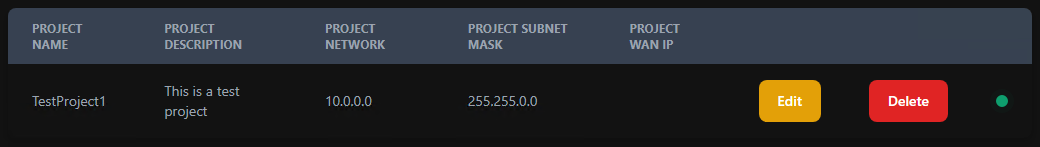
\includegraphics[scale=0.8]{images/test-project-1.png}
    \caption{Test Project 1 created successfully}
    \label{fig:test-project-1}
\end{figure}

As can be seen, the project has been allocated a subnet of 10.0.0.0/16. This can be used to set IP addresses on the two test \gls{vm}s. The IP addresses of 10.0.1.1 and 10.0.1.2 were chosen respectively. After assigning the IP addresses, the test \gls{vm}s were able to ping each other. Figures \ref{fig:test-project-1-ping-1} and \ref{fig:test-project-1-ping-2} show the successful ping test, showing that the \gls{aci} fabric is being provisioned correctly.

\begin{figure}[H]
    \centering
    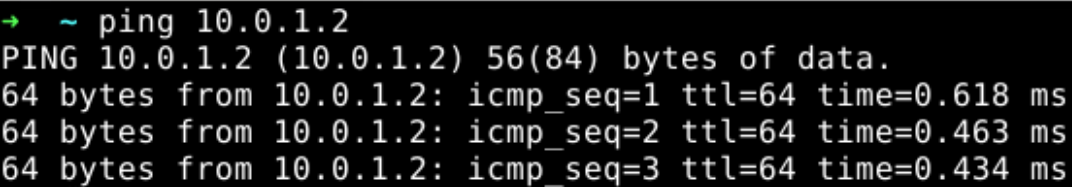
\includegraphics[scale=0.7]{images/test-project-1-ping.png}
    \caption{Test VM 1 pinging Test VM 2}
    \label{fig:test-project-1-ping-1}
\end{figure}

\begin{figure}[H]
    \centering
    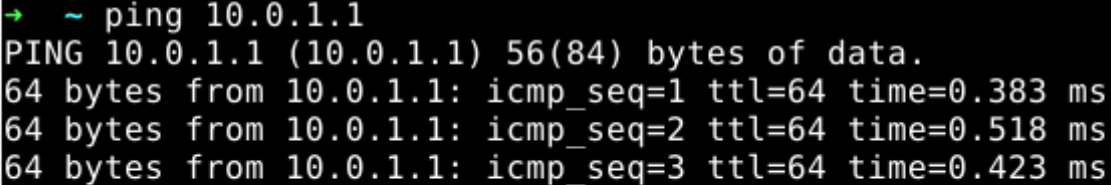
\includegraphics[scale=0.7]{images/test-project-1-ping-2.png}
    \caption{Test VM 2 pinging Test VM 1}
    \label{fig:test-project-1-ping-2}
\end{figure}

The next test was to ping the internet from the test \gls{vm}s. This was done by pinging the IP address of both Cloudflare and Google DNS, which is shown in figure \ref{fig:test-project-1-ping-internet}. This shows that the virtual router is being provisioned correctly.

\begin{figure}[H]
    \centering
    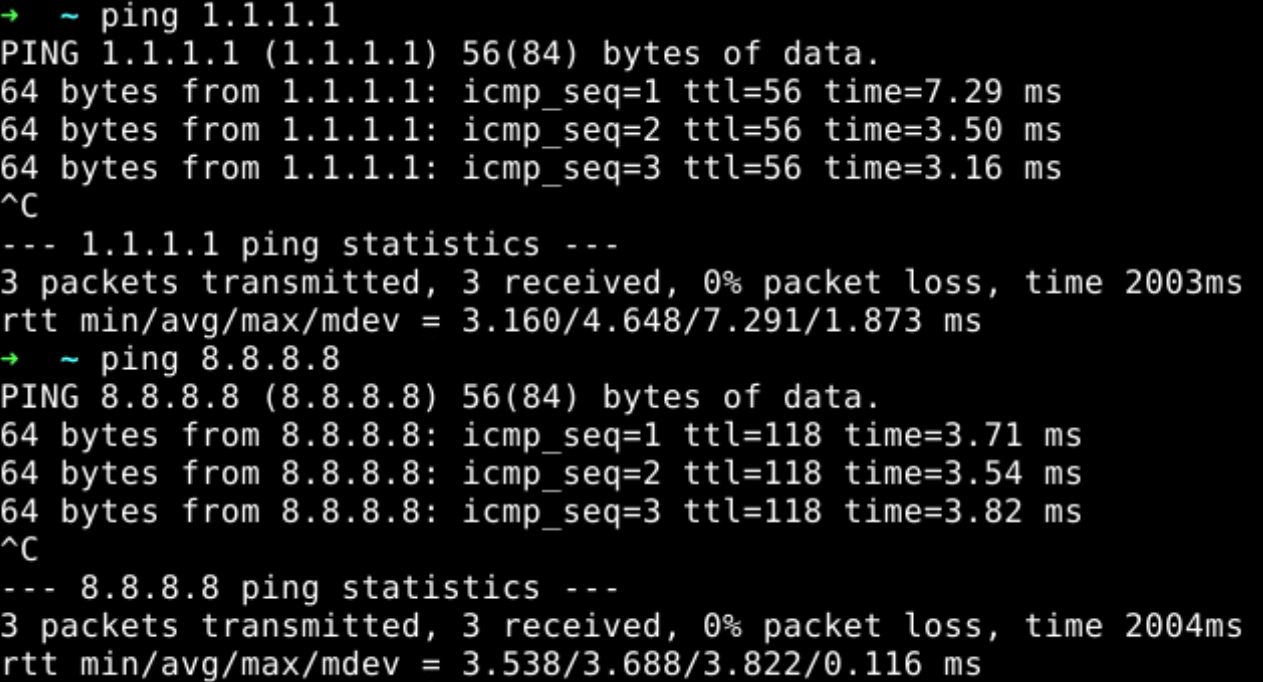
\includegraphics[scale=0.5]{images/test-project-1-ping-internet.png}
    \caption{Test VM 1 pinging the internet}
    \label{fig:test-project-1-ping-internet}
\end{figure}

\section{Terminal Server Reachability}

The terminal servers are automatically allocated the first available IP addresses sequentially in the order of the racks. In the case of this test project which has been allocated the network of 10.0.0.0/16, the addresses of the terminal servers will be 10.0.0.1 and 10.0.0.2 respectively. When pinging, 10.0.0.1 responded, however, TS-2 - 10.0.0.2 did not. Upon checking the configuration of TS-2, it was noted that no sub-interface configuration had been applied to the device. Figure \ref{fig:terminal-server-provision-bug} shows the problematic configuration script.

\begin{figure}[H]
    \begin{lstlisting}[basicstyle=\scriptsize]
        $project = Project::with('racks.terminalServer', 'vlan')->find($this->projectId);
        foreach ($project->racks as $key => $rack) {
            if ($rack->terminalServer !== null) {
                $iosXE = new IOSXEClient($rack->terminalServer->ip,
                  $rack->terminalServer->username, $rack->terminalServer->password);
                if ($iosXE->connectionTest()) {
                    if ($iosXE->setSubInterface($this->firstUsableIP($project->network,
                      $project->subnet_mask, $key), $project->subnet_mask,
                       $project->vlan->vlan_id, $rack->terminalServer->uplink_port)) {
                        $iosXE->save($rack->terminalServer->username,
                          $rack->terminalServer->password);

                        return true;
                    }
                }
            }
        }
        return false;

    \end{lstlisting}
    \caption{Terminal Server Provisioning Script}
    \label{fig:terminal-server-provision-bug}
\end{figure}

The issue is that the return statement will break the execution after the successful provisioning of the first terminal server, hence only the first was being provisioned. The fix was to remove the return statement to after the foreach loop. Figure \ref{fig:terminal-server-ping} shows the connectivity which was successful after the bug fix.

\begin{figure}[H]
    \centering
    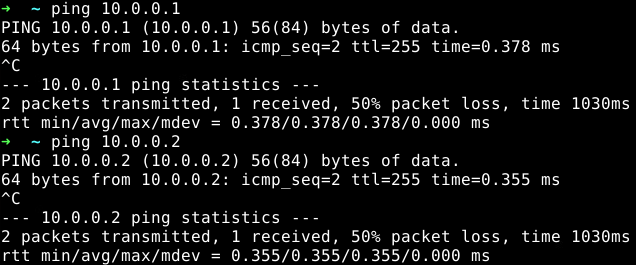
\includegraphics[scale=1.5]{images/terminal-server-ping.png}
    \caption{Test VM 1 pinging TS-1 and 2}
    \label{fig:terminal-server-ping}
\end{figure}

\section{Multiple Projects}
To test intra-project communication is not possible, so the original test project was reduced to occupying one rack. A new project was created, consuming the remaining two racks. This will test to ensure that the automation platform correctly provisions the fabric and terminal servers for each project and that the automation script correctly deallocates and allocates racks, even with existing projects. Figures \ref{fig:two-projects} and \ref{fig:two-projects-racks} show the new project, which has been successfully added to the platform.

\begin{figure}[H]
    \centering
    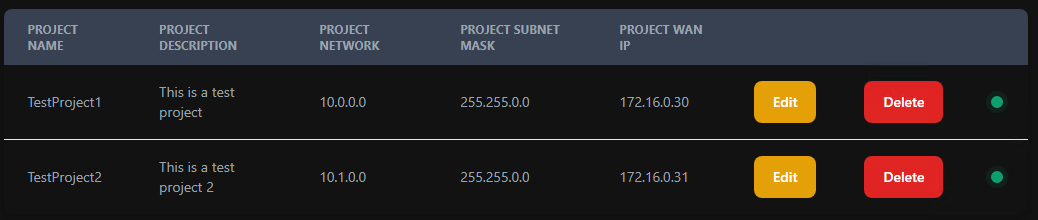
\includegraphics[scale=1]{images/two-projects.png}
    \caption{Test Project 2 created successfully}
    \label{fig:two-projects}
\end{figure}

\begin{figure}[H]
    \centering
    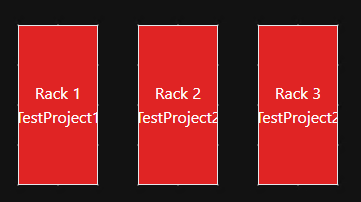
\includegraphics[scale=1.2]{images/two-projects-racks.png}
    \caption{Rack Allocation with additional project}
    \label{fig:two-projects-racks}
\end{figure}

Test \gls{vm}s 1 and 2 were reconfigured with the IP addresses of 10.1.1.1 and 10.1.1.2 respectively to account for the change in the subnet. A ping test was performed between the two \gls{vm}s, which was successful. Figure \ref{fig:two-projects-ping} shows the successful ping test.

\begin{figure}[H]
    \centering
    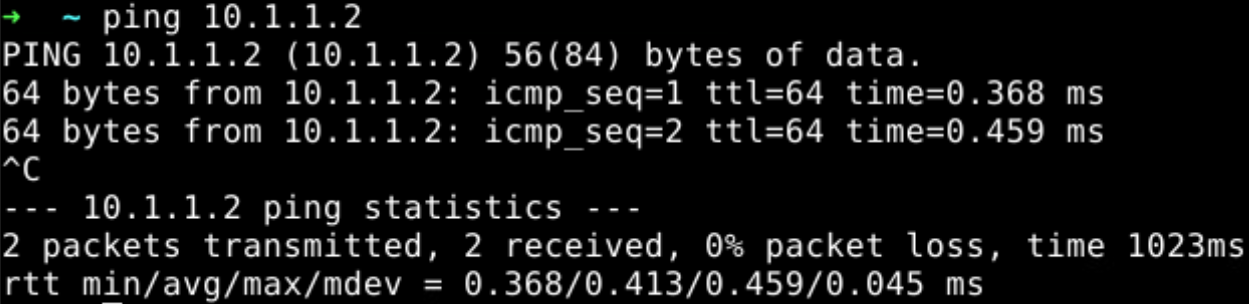
\includegraphics[scale=0.8]{images/two-projects-ping.png}
    \caption{Test VM 3 pinging Test VM 2}
    \label{fig:two-projects-ping}
\end{figure}

The reachability of TS-2, which is now in the second project was also tested, via \gls{ssh} from Test \gls{vm} 3. This was successful, as shown in figure \ref{fig:two-projects-ssh}. This shows that the automation platform correctly allocates and deallocates racks, even with existing projects.

\begin{figure}[H]
    \centering
    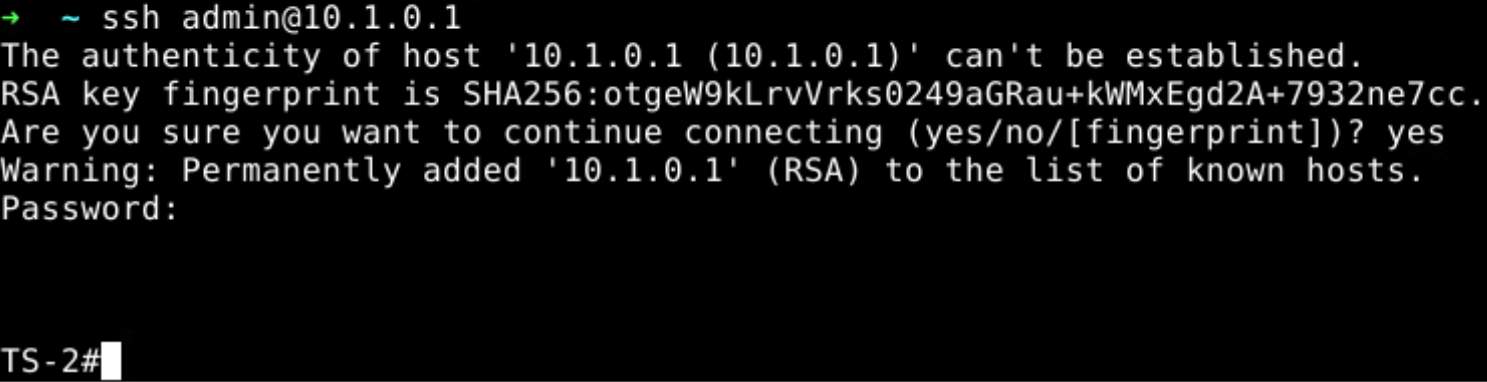
\includegraphics[scale=0.7]{images/two-projects-ssh.png}
    \caption{Test VM 3 pinging TS-2}
    \label{fig:two-projects-ssh}
\end{figure}

To verify the fact that the projects do not have any communication between them, the IP address of Test \gls{vm} 2 was reverted to the 10.0.0.0/16 subnet, and 10.0.1.1 was pinged, which is the IP of test \gls{vm} 1. As seen in figure \ref{fig:inter-project-communication} the ping test has failed, verifying that the projects are isolated from one another.

\begin{figure}[H]
    \centering
    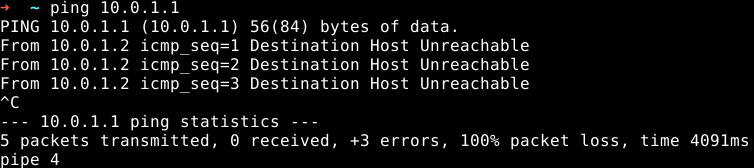
\includegraphics[scale=1.2]{images/inter-project-communication.png}
    \caption{Test VM 2 pinging Test VM 1 from different projects}
    \label{fig:inter-project-communication}
\end{figure}

\section{Project Deletion}
To verify that the correct fabric policies, terminal server interfaces and project router \gls{vm} are correctly deleted, both projects were deleted. The configuration of the \gls{aci} fabric was then inspected along with vCenter inventory. Figure \ref{fig:aci-empty-tenants} shows that the tenants have been deleted automatically. Figure \ref{fig:aci-empty-interface-policy} shows that the interface policies have been deleted correctly. Figure \ref{fig:empty-vcenter} shows the project \gls{vm}s have been cleared up appropriately.


\begin{figure}[H]
    \centering
    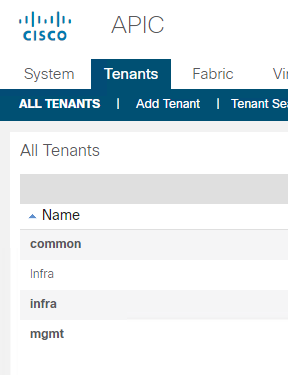
\includegraphics[scale=1.2]{images/aci-empty-tenants.png}
    \caption{ACI Fabric Tenants}
    \label{fig:aci-empty-tenants}
\end{figure}

\begin{figure}[H]
    \centering
    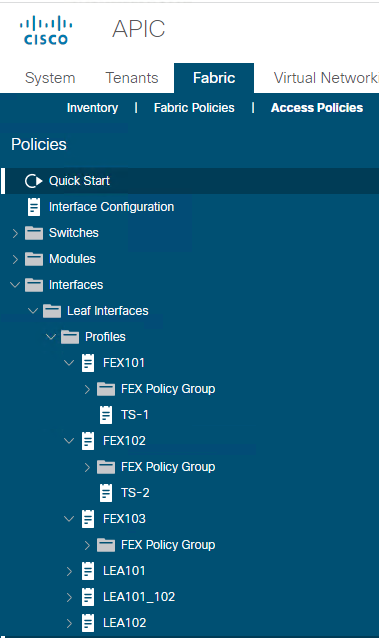
\includegraphics[scale=1.2]{images/aci-empty-interface-policy.png}
    \caption{ACI Fabric Interface Policies}
    \label{fig:aci-empty-interface-policy}
\end{figure}

\begin{figure}[H]
    \centering
    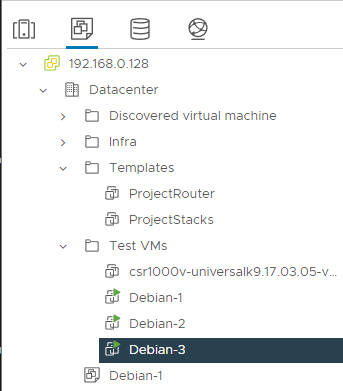
\includegraphics[scale=1.2]{images/empty-vcenter.png}
    \caption{vCenter Inventory}
    \label{fig:empty-vcenter}
\end{figure}
